In this section we design a framework to collect and analyze addtional data from the point of view of a virtual guest system. 
First, we define the new layers of abstraction in virtual environments.  
Then we identify the virtual resources that require additional information from these layers.
For measuring I/O performance in a virtual guest, we describe the following method to collect and analyze the additional data:
\begin {enumerate}
  \item Identify the relevant performance counters for a resource.
  \item A method to calculate the overhead of virtualization without interference.
  \item A method to analyze performance of a guest machine which may be experiencing degredation from external interference.
\end{enumerate}

% 1 Define the new layers of abstraction virtual environments.
\subsection{Abstraction Layers}
As we have previously stated, a virtual machine could behave unexpectedly due to interference and overhead from virtualization.
Without virtualization, the problem could be in the application, OS, or hardware.  
In a virtual environment, the hypervisor and external guests also need to be considered as a cause of the problem (Table \ref{tab:layers}).  
The hypervisor provides the virtual resources to the guest and controls access to the physical hardware.  
Since the guest machine can only access the hardware through the hypervisor, it will have some performance overhead. 
An external guest machine may also cause interference by competing for resources with other running guest machines.  
Performance problems can be caused by the hypervisor or external guest and needs to be considered when trying to determine the root cause of the problem.

\begin{table}[h]
\begin{tabular}{ l p{10cm} }
  Layer & Definition \\
  \hline
  Application & Includes all code and libraries running in user space. \\
  OS & Includes all kernel code and device drivers. \\
  \textbf{Extrenal Guest} & An external virtual system. \\
  \textbf{Hypervisor} & The hypervisor and VMM to manage the guest domains. \\
  Hardare & Physical hardware. \\
  \hline
\end{tabular}
\caption{New layers \emph{Hypervisor} and \emph{External Guest} for virtualizataion}
\label{tab:layers}
\end{table}

% 2 Identify resources which are difficult to measure usage.
\subsection{Resources}
Now we define the virtual resources available to the guest OS and applications.
In a virtual environment, the resources allocated to a guest machine are an abstraction of the physical resources available.  
If the physical resource is used by other layers of virtualization the guest machine will not have complete access to the physical resource.    
Additional information is needed from hypervisor about the physical resource so that the administrator, OS, or application can make better decisions about the availability of the resource. 

\begin{table}[h]
  \begin{tabular}{ l p{10cm} }
    Resource & Definition \\
    \hline
    CPU & The virtual core allocated to the guest \\
    Memory & The virtual RAM allocated to the guest \\
    Disk I/O & The virtual block disk I/O system \\
    Net I/O & The virtual network I/O system \\
    \hline
  \end{tabular}
\caption{Virtual resources which may experience interference from hypervisor or external guest.}
\label{tab:resources}
\end{table}

% 3 Identify the performance counters which can be used to measure I/O performance on a virtual guest machine.
\subsection{Performance Counters}
Performance counters are used by system administrators and developers to show how the resources are utilized and determine if the application is bound by Memory, I/O, or CPU (Table \ref{tab:resources}).  
In other words, adding additional Memory, I/O, or CPU would improve application performance. 
On a Linux OS most of the utilities used to identify resource usage comes from the /proc filesystem \cite{proc}. 
For example the \emph{sar -d} command will show block device statistics such as transfers/sec, reads/sec, and writes/sec, as well as many other statistics.  
Similar GUI are available on Microsoft Windows OS through perfmon.exe and an API in the Windows Performance Toolkit \cite{winperf}. 

\begin{comment}
The hypervisor divides the physical resource into virtual resources for each guest.  
Additionally, each resource may be shared between multiple guests by overcommitting the resource.  
When a guest system views statistics about a resource, part of the information is missing from the guest application.  
Interference from the hypervisor and external guests need to be passed to the guest virtual machine about the true performance of the resource. 
\end{comment}

\indent To monitor resource usage of applications and the kernel, administration tools will read these counters over some period of time.  
Then a tool will display the output in some report or graph to show how the system resources are used.
For example to display I/O reads per second every 5 seconds a tool may do the following:
\begin{figure}[h]
\begin{algorithmic}[H]
 \STATE $interval \gets 5$
 \STATE $counter \gets$  Disk Read
 \STATE $pre \gets READ counter$ 
 \LOOP
    \STATE $SLEEP  interval$
    \STATE $post \gets READ  counter$
    \STATE $result \gets (post - pre)/interval$
    \STATE $PRINT  result$
    \STATE $pre \gets post$ 
 \ENDLOOP
\end{algorithmic}
\caption{Method for any system (physical server, virtual server, or hypervisor) to collect performance information.  This example displays the count of \emph{disk reads} every 5 seconds}
\label{alg1}
\end{figure}

\indent For each resource available on a most operating systems, there are many OS level statistics collected about those resources.  It is important to indentify the resources used, and the performance counters for each resource.  
For our experiments we use I/O and virtual memory statistics, but other statistics could be collected for CPU or network resource usage.

% 4 A method to calculate the overhead and theoritical maximum performance using an offline modeling technique.
\subsection{Virtualization Overhead}
For each virtual resource (Table \ref{tab:resources}) there is a performance cost to making that resource virtualized.  If the guest had direct access to the hardware the virtualization cost would be 0.  Since most system calls from the guest kernel needs to go through the hypervisor, we need to account for this additional time, even when the \emph{external guest} layer does not cause interference. 

\indent Several researchers \cite{cherkasova, huber1} have called this cost the \emph{overhead}, and have quantified the overhead for a given configuration.  This research used an offline modeling technique by running a benchmark with and without virtualization.  By taking the difference of these two benchmarks they can calculate the overhead.
This type of test is good for generalizing the performance of the hypervisor for a given configuration.
The problem with this technique is that physical servers would need to be provisioned for this exercise.  Any configuration changes in hardware or anywhere in the software stack, may require a new test.  

\indent Before a guest application is run in a virtualized environment, we need to calculate the \emph{overhead} in that environment.  This only needs to be done once per configuration.  In large scale datacenters and cloud systems, templates are usually created before virtual machines are used in production.  A template is a complete snapshot image of a virtual machine that has been built and tested to meet some need.  For example a Redhat 6.2 system with an Apache web server may need to be used on several machines.  A system could be built, tuned, and tested for that enviroment and then made into a template.  Future users can deploy a new virtual machine from that template.  We are suggesting to calculate the overhead from virtualization when it is made into a template.  

\indent To calculate the virtualization overhead, create a single virtual machine with dedicated resources on isolated hardware.  
Only the virtual machine should be deployed without any other guests running and causing interference, as we only want to measure overhead from the hypervisor.  

\indent Next we need to find a test load that will stress the resource (Table \ref{tab:resources}).   
There are many performance benchmarks that can be used \cite{katcher, tikotekar, hplBench}. 
It may be possible to generate a load that will stress I/O, memory, and CPU, but it is best to stress them separately since other interference could mislead results.  
Then place the load on the virtual machine and begin monitoring the performane counters for that resource using the algorithm in Figure \ref{alg1} in BOTH the guest OS and hypervisor. 

\begin{figure}[!h]
  \begin{center}
  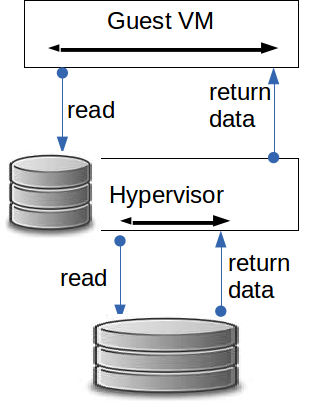
\includegraphics[width=2in]{images/ReadOperation.png}
  \caption{The total time to read from a virtualized disk.  Both the guest and the hypervisor account this statistic in their kernel data.}
  \label{readOp}
  \end{center}
\end{figure}

\indent For a given performance counter and some time interval, we count the hypervisor \emph{count\textsubscript{H}} and the guest \emph{count\textsubscript{G}}.  
We assert that for counters that track the time spent using a resource, the overhead is the additional time spent in the guest.    
The guest will report the total time, which is the time the guest sent the request until it was returned.
The hypervisor will report the time spent to actually read from the physical block device.
For example:  On a Linux guest we can measure \emph{the time spent reading (ms)} from block devices \cite{diskstats}.  We can also read this counter in the hypervisor on Xen and other virtualization platforms.
The guest may spend 200ms and 150ms is used for the task in the hypervisor then the overhead to virtualize the task is 50ms or 25\% of the total time.

\begin{equation}
  Overhead_V = \frac{count_G - count_H}{count_G} 
\end{equation}

% A method to analyze performance of a guest machine which may be experiencing degredation from external interference.
\subsection{Detecting Interference}
In order to collect performance metrics (such as reads/second and writes/second) with a complete view of the resource, we need a method to calculate how much of that resource is used by the external guests and the hypervisor overhead.  
At each layer and each resource, data and statistics need to be shared and aggregated to determine why the application may be degraded.

\indent When a tool runs in the userspace of guest machine to get resource usage, the guest OS should request information about the usage of the resource from the hypervisor and external guests.  Since the guest has previously collected the \emph{overhead}, then the guest virtual machine can determine if the resource is degraded by examining the sum of all of counters from the virtual machines and calculating the overhead from all of the virtual machines.

\begin{enumerate}
	\item Guest tool requests OS permance counter statistics.
	\item Guest OS forwards request to hypervisor.
	\item Hypervisor forwards request to all guests.
	\item Hypervisor begins monitoring for specified time and waits determined time.
	\item Each Guest responds with individual statistics.
	\item Hypervisor calculates $Overhead_{Vall}$ (Equation 2) of resource used.
	\item Hypervisor returns $Overhead_{Vall}$ to original requestor.
	\item Guest calculates the $Interference$ (Equation 3).
\end{enumerate}

\indent Since the guest has previously calculated $ Overhead_V $ we can use that information to calculate the interference when multiple guests are run concurrently $ Overhead_{Vall} $.  If all \emph{n} guests have been modified to collect and pass information to the hypervisor, each guest can reply with their counters when asked by the hypervisor.  It is important that all guests and the hypervisor start and stop counting concurrently to provide accurate results.  

\[ Count_{Gall} = \sum_{i=1}^n{count_G} \] 
\begin{equation}
Overhead_{Vall} = \frac{count_{Gall} - count_H}{count_{Gall}} 
\label{eq2}
\end{equation}

\indent We can see that when the number of guests machines is 1 (as when we collected the overhead with 1 machine), this is exactly as equation 1.  After the hypervisor calculates the count and overhead for all machines running and passes this information to the original guest, the guest can then calculate the interference.  
The interference from other virtual machines $Interference_V$ is calculated by subtracting the overhead from all guests from the original overhead found without any external interference. 

\begin{equation}
Interference_V = Overhead_{Vall} - Overhead_V
\label{eq3}
\end{equation}

\indent As an example: the userspace tool \emph{iostat} reads disk performance counters in /proc/diskstats and will report transfers, bytes read, and bytes written per second.  If an application was experiencing I/O performance problems this would be a tool an administrator or application developer may monitor.  Without knowing the interference this could be misleading as to the root cause of the problem.  The following example shows a possible output from the perspective of the running guest when experienceing I/O interference from external guest machines.
\begin{figure}[h]
\begin{Verbatim}
Device:  tps    kB_read/s    kB_wrtn/s
sda   577.20     41388.00    148073.00
 virtual I/O interference 22.4%     
\end{Verbatim}
\label{fig:iostat}
\caption{Example:  \emph{iostat} with additional information from hypervisor calcuated interference}
\end{figure}

\begin{comment}
\subsection{Disk Pinning}
Disk pinning may be a solution for multiple I/O bound guest appliations running in a virtual system.  Several papers have demonstrated the effects of core pinning or \emph{core affinity} for CPU bound applications, which can reduce the load on the hypervisor and prevent cache contention.  Similarly, a multiple I/O bound guests may use a single disk excessivley causing interference and degreaded performance.  By increasing the number of physical spindles, multiple random disk seeks can occur concurrently.  By setting physical disks to specific virtual guests, we can reduce I/O interference from multiple guests.  For applications that are bound by virtual I/O resources, it may be better to share cores and separate physical disks for each virtual machine.  At some point assigning a dedicated physical resource to guest machines minimizes the benefits of virtualizaion.  It should be the task of the administrator to decide how the physical resources are used based on the need.
\end{comment}
